\documentclass[a4paper,12pt]{article}
\usepackage[top = 2.5cm, bottom = 2.5cm, left = 2.5cm, right = 2.5cm]{geometry}
\usepackage[T1]{fontenc}
\usepackage[utf8]{inputenc}
\usepackage{multirow} 
\usepackage{booktabs} 
\usepackage{graphicx}
\usepackage[spanish]{babel}
\usepackage{setspace}
\setlength{\parindent}{0in}
\usepackage{float}
\usepackage{fancyhdr}
\usepackage{amsmath}
\usepackage{amssymb}
\usepackage{amsthm}
\usepackage[numbers]{natbib}
\newcommand\Mycite[1]{%
	\citeauthor{#1}~[\citeyear{#1}]}
\usepackage{graphicx}
\usepackage{subcaption}
\usepackage{booktabs}
\usepackage{etoolbox}
\usepackage{minibox}
\usepackage{hyperref}
\usepackage{xcolor}
\usepackage[skins]{tcolorbox}
%---------------------------

\newtcolorbox{cajita}[1][]{
	 #1
}

\newenvironment{sol}
{\renewcommand\qedsymbol{$\square$}\begin{proof}[\textbf{Solución.}]}
	{\end{proof}}

\newenvironment{dem}
{\renewcommand\qedsymbol{$\blacksquare$}\begin{proof}[\textbf{Demostración.}]}
	{\end{proof}}

\newtheorem{problema}{Problema}
\newtheorem{definicion}{Definición}
\newtheorem{ejemplo}{Ejemplo}
\newtheorem{teorema}{Teorema}
\newtheorem{corolario}{Corolario}[teorema]
\newtheorem{lema}[teorema]{Lema}
\newtheorem{prop}{Proposición}
\newtheorem*{nota}{\textbf{NOTA}}
\renewcommand\qedsymbol{$\blacksquare$}
\usepackage{svg}
\usepackage{pgfplots}
\pgfplotsset{compat=1.11}

\usepackage{tikz}
\usetikzlibrary{calc}

\usetikzlibrary{patterns}
\usepackage[framemethod=default]{mdframed}
\global\mdfdefinestyle{exampledefault}{%
linecolor=lightgray,linewidth=1pt,%
leftmargin=1cm,rightmargin=1cm,
}




\newenvironment{noter}[1]{%
\mdfsetup{%
frametitle={\tikz\node[fill=white,rectangle,inner sep=0pt,outer sep=0pt]{#1};},
frametitleaboveskip=-0.5\ht\strutbox,
frametitlealignment=\raggedright
}%
\begin{mdframed}[style=exampledefault]
}{\end{mdframed}}
\newcommand{\linea}{\noindent\rule{\textwidth}{3pt}}
\newcommand{\linita}{\noindent\rule{\textwidth}{1pt}}

\AtBeginEnvironment{align}{\setcounter{equation}{0}}
\pagestyle{fancy}

\fancyhf{}









%----------------------------------------------------------
\lhead{\footnotesize Geometría diferencial}
\rhead{\footnotesize  Rudik Roberto Rompich}
\cfoot{\footnotesize \thepage}


%--------------------------

\begin{document}
 \thispagestyle{empty} 
    \begin{tabular}{p{15.5cm}}
    \begin{tabbing}
    \textbf{Universidad del Valle de Guatemala} \\
    Departamento de Matemática\\
    Licenciatura en Matemática Aplicada\\\\
   \textbf{Estudiante:} Rudik Roberto Rompich\\
   \textbf{Correo:}  \href{mailto:rom19857@uvg.edu.gt}{rom19857@uvg.edu.gt}\\
   \textbf{Carné:} 19857
    \end{tabbing}
    \begin{center}
        Geometría diferencial - Catedrático: Alan Reyes\\
        \today
    \end{center}\\
    \hline
    \\
    \end{tabular} 
    \vspace*{0.3cm} 
    \begin{center} 
    {\Large \bf  Tarea
} 
        \vspace{2mm}
    \end{center}
    \vspace{0.4cm}
%--------------------------

\begin{problema}
    Mostrar que el cilindro $\left\{(x, y, z) \in \mathbb{R}^3: x^2+y^2=1\right\}$ es una superficie regular, y encuentre parametrizaciones que cubran dicha superficie. Mostrar que el cono $C: x^2+y^2=z^2$ no es una superficie regular.
    \begin{proof}
        En clase se demostró la siguiente proposición: 
        \begin{cajita}
            \begin{prop}

                Sea $f: U \subseteq  \mathbb{R}^3 \to \mathbb{R}$ una función diferenciable y sea $a\in f(U)$
                un valor regular de $f$. Entonces, $S = f^{-1}(a)$ es una superficie regular.
                        \end{prop}
        \end{cajita}
        Entonces, sea $f: U\subseteq \mathbb{R}^3\to \mathbb{R}\ni$
        $$f(x,y,z)= x^2+y^2-1$$
        En donde su gradiente igualado a cero nos indica los puntos críticos
        $$dF =\left(2x\quad 2y \quad 0\right)=0$$
        que tienen la forma de $(x=0,y=0,z)$, es decir el conjunto de puntos críticos es $\left\{(0,0,z)\in \mathbb{R}^3| x,y,z\in U\subseteq\mathbb{R}\right\}$, entonces el conjunto de valores críticos es $\{f(0,0,z)=0^2+0^2-1\in \mathbb{R}|(x,y,z)\in U\subseteq\mathbb{R}^3\}$. Por lo que los valores regulares, son los que tienen la forma $$\mathbb{R}-\{f(0,0,z)=-1\in \mathbb{R}|(x,y,z)\in U\subseteq\mathbb{R}^3\}$$
        Es decir, un valor regular es $0$. Tal que 
        \begin{align*}
            f^{-1}(0) &=\left\{f(x,y,z)=0| (x,y,z)\in U\subseteq \mathbb{R}^3\right\}\\
            &= \left\{x^2+y^2-1=0| (x,y,z)\in U\subseteq \mathbb{R}^3\right\}\\
            &= \left\{x^2+y^2=1| (x,y,z)\in U\subseteq \mathbb{R}^3\right\}\\
        \end{align*}
        Por lo que se cumple la proposición y se demuestra que  el cilindro $\left\{(x, y, z) \in \mathbb{R}^3: x^2+y^2=1\right\}$ es una superficie regular.

        Para la segunda parte, un cilindro se puede parametrizar como $x_1:W\to \mathbb{R}^3$
        $$x_1(u,v)=\left(\cos u, \sin u, v\right),\quad W=\left\{(u,v)\in \mathbb{R}^3,0<u<2\pi,a<v<b\right\},$$
        
        El cual ya se había demostrado en clase (el caso general) que es una superficie regular. 

        ---------------------------------------------------------------------------------------------------------------------

        Por último, hay que demostrar que $C: x^2+y^2=z^2$ no es una superficie regular. Por reducción al absurdo, supóngase que $C$ es una superficie regular. Entonces, sea $f: U\subseteq \mathbb{R}^3\to \mathbb{R}\ni$
        $$f(x,y,z)= x^2+y^2-z^2,$$
        tal que la superficie regular se puede representar como:
        $$C=\left\{f(x,y,z)=0| (x,y,z)\in U\subseteq \mathbb{R}^3\right\}$$

        En donde su gradiente igualado a cero nos indica los puntos críticos
        $$dF =\left( 2x\quad 2y \quad -2z\right)=0$$
        que tienen la forma de $(x=0,y=0,z=0)$, es decir el conjunto de puntos críticos es $\left\{(0,0,0)\in \mathbb{R}^3| x,y,z\in C\subseteq\mathbb{R}\right\}$. Ahora bien, estamos negando la definición de ser superficie regular, ya que tenemos un punto $(0,0,0)\in C$, pero que hace que $dF$ se anule, entonces no cumple con la condición de regularidad. 
    \end{proof}
\end{problema}

\begin{problema}
    Sea $f(x, y, z)=z^2$. Muestre que 0 no es un valor regular de $f$ y que aún así, $f^{-1}(0)$ es una superficie regular.
    \begin{dem}
        Sea $f: U\subseteq \mathbb{R}^3\to \mathbb{R}\ni$
        $$f(x,y,z)= z^2,$$
        En donde su gradiente igualado a cero nos indica los puntos críticos
        $$dF =\left(0\quad 0 \quad 2z\right)=0$$
        que tienen la forma de $(x,y,z=0)$, es decir el conjunto de puntos críticos es 
        $$\left\{(x,y,0)\in \mathbb{R}^3| x,y,z\in U\subseteq\mathbb{R}\right\},$$ entonces el conjunto de valores críticos es $$\{f(x,y,z)=0^2=0\in \mathbb{R}|(x,y,z)\in U\subseteq\mathbb{R}^3\}.$$
        Por lo que los valores regulares, son los que tienen la forma $$\mathbb{R}-\{f(x,y,z)=0^2=0\in \mathbb{R}|(x,y,z)\in U\subseteq\mathbb{R}^3\}$$
        Es decir, que el $0$ no es un valor regular de $f$. Por otra parte, en clase se había demostrado que el plano es una superficie regular, por lo que $f^{-1}(0)$ es una superficie regular.  
    \end{dem}

\end{problema}


\begin{problema}
    Sea $f(x, y, z)=(x+y+z-1)^2$.
    \begin{enumerate}
        \item Localizar los puntos críticos y valores críticos de $f$.
        \begin{sol}
            Sea $f: U\subseteq \mathbb{R}^3\to \mathbb{R}\ni$
        $$f(x,y,z)= (x+y+z-1)^2,$$
        En donde su gradiente igualado a cero nos indica los puntos críticos
        $$dF =\left(2(x+y+z-1)\quad 2(x+y+z-1) \quad 2(x+y+z-1)\right)=0,$$
        es decir el conjunto de puntos críticos es 
        $$\left\{(x,y,x)\in \mathbb{R}^3| x+y+z=1\right\},$$ entonces el conjunto de valores críticos es $$\{f(x,y,z)=(\underbrace{x+y+z}_1-1)^2=0\in \mathbb{R}|(x,y,z)\in U\subseteq\mathbb{R}^3\}.$$
        \end{sol}
        \item ¿Para qué valores de $c$ el conjunto $f(x, y, z)=c$ es una superficie regular?
        \begin{sol}
            Basado en el inciso anterior, los valores regulares, son los que tienen la forma $$\mathbb{R}-\{f(x,y,z)=0\in \mathbb{R}|(x,y,z)\in U\subseteq\mathbb{R}^3\}$$
            Es decir, un valor regular es $c\neq0$. Tal que 
            \begin{align*}
                f^{-1}(c) &=\left\{f(x,y,z)=c| (x,y,z)\in U\subseteq \mathbb{R}^3\right\}\\
                &= \left\{x^2+y^2-1=c| (x,y,z)\in U\subseteq \mathbb{R}^3\right\}\\
                &= \left\{x^2+y^2=c+1| (x,y,z)\in U\subseteq \mathbb{R}^3\right\}\\
            \end{align*}
        \end{sol}
        \item Responder las preguntas en (a) y (b) para la función $g(x, y, z)=x y z^2$.
        \begin{sol}
            Sea $f: U\subseteq \mathbb{R}^3\to \mathbb{R}\ni$
        $$f(x,y,z)= xyz^2,$$
        En donde su gradiente igualado a cero nos indica los puntos críticos
        $$dF =\left(yz^2\quad xz^2 \quad 2zxy\right)=0,$$
        es decir el conjunto de puntos críticos es 
        $$\left\{(x,y,x)\in \mathbb{R}^3| (z=0)\vee (x=0\wedge y=0)\right\},$$ entonces el conjunto de valores críticos es $$\{f(x,y,z)=0\in \mathbb{R}|(x,y,z)\in U\subseteq\mathbb{R}^3\}.$$
        Entonces los valores regulares, son los que tienen la forma $$\mathbb{R}-\{f(x,y,z)=0\in \mathbb{R}|(x,y,z)\in U\subseteq\mathbb{R}^3\}$$
        Es decir, un valor regular es $c\neq0$. Tal que 
        \begin{align*}
            f^{-1}(c) &=\left\{f(x,y,z)=c| (x,y,z)\in U\subseteq \mathbb{R}^3\right\}\\
            &= \left\{xyz^2=c| (x,y,z)\in U\subseteq \mathbb{R}^3\right\}
        \end{align*}
        \end{sol}
    \end{enumerate}


\end{problema}

\begin{problema}
    Probar que $\mathbf{x}: U \subseteq \mathbb{R}^2 \rightarrow \mathbb{R}^3$ dada por
$$
\mathbf{x}(u, v)=(a \sin u \cos v, b \sin u \sin v, c \cos u), \quad a, b, c \neq 0,
$$
con $0<u<\pi, 0<v<2 \pi$, es una parametrización para el elipsoide $\frac{x^2}{a^2}+\frac{y^2}{b^2}+\frac{z^2}{c^2}=1$. Describir geométricamente las curvas $u=$ const y $v=$ const. sobre el elipsoide.
\begin{sol}
    A probar: un subconjunto $S \subset \mathbb{R}^3$ es una superficie regular si para cada punto $p \in S$, existe una vecindad $V$ en $S$ y un mapa $\mathbf{x}: U \subset \mathbb{R}^2 \rightarrow V$ tal que: (1) $\mathbf{x}$ es diferenciable, (2) $\mathbf{x}$ es un homomorfismo (3) y la derivada $d\mathbf{x}_q: \mathbb{R}^2 \rightarrow T_p(\mathbb{R}^3)$ es inyectiva para cada $q\in U$.
    Pero primero, hacemos la verificación trivial: 
    $$\begin{aligned} \frac{(a \sin u \cos v)^2}{a^2}+\frac{(b \sin u \sin v)^2}{b^2}+\frac{(c \cos u)^2}{c^2} & =\sin ^2 u \cos ^2 v+\sin ^2 u \sin ^2 v+\cos ^2 u \\ & =\sin ^2 u\left(\cos ^2 v+\sin ^2 v\right)+\cos ^2 v \\ & =\sin ^2 u \cdot 1+\cos ^2 v=1\end{aligned}$$
    \begin{itemize}
        \item $x$ es diferenciable. Sea  $$ \frac{\partial x}{\partial u}=a \cos u \cos v,\quad \frac{\partial x}{\partial v}=-a \sin u \sin v, $$ $$ \frac{\partial y}{\partial u}=b \cos u \sin v,\quad \frac{\partial y}{\partial v}=b \sin u \cos v, $$  $$ \frac{\partial z}{\partial u}=-c \sin u,\quad \frac{\partial z}{\partial v}= 0 $$
        Por lo que sus derivadas parciales son continuas y de clase $C^\infty$. Por lo tanto, $x$ es diferenciable. 
        \item  $x$ es un homomorfismo. Nótese que $x$ es continua, ya que sus componente lo son. Ahora, verificaremos que es biyectiva: 
        \begin{enumerate}
            \item Inyectiva. Sea 
            \begin{align*}
                x(u,v) &= x(u',v')\\
                (a \sin u \cos v, b \sin u \sin v, c \cos u) &= (a \sin u' \cos v', b \sin u' \sin v', c \cos u')\\
            \end{align*}
            De esto tenemos, 
            \begin{align*}
                \sin u \cos v &= \sin u' \cos v'\\
                \sin u \sin v &= \sin u' \sin v'\\
                \cos u &= \cos u'
            \end{align*}
            Entonces:
            \begin{align*}
                \sin u  &= \sin u'\\
                \sin v &= \sin v'\\
                \cos u &= \cos u'
            \end{align*}
            Lo que nos permite concluir, 
            $$(u,v)=(u',v')$$
            \item Sobreyectividad. Para cada $(u,v,w)\in \mathbb{R}^3, \exists (u,v)\in \mathbb{R}^2$, tal que la regla de asignación se cumple.   
        \end{enumerate}
        
        Ahora, nos falta verificar que la inversa es continua. Debemos resolver el sistema de ecuaciones dado por $\mathbf{x}(u,v) = (a \sin u \cos v, b \sin u \sin v, c \cos u)=(x,y,z)$. Esto nos da: 
        
        $$ u = \cos^{-1}\left(\frac{z}{c}\right), $$ 
        y 
        $$ v = \begin{cases} \sin^{-1}\left(\frac{y}{b\sin u}\right) & x > 0 \\\pi - \sin^{-1}\left(\frac{y}{b\sin u}\right) & x < 0. \end{cases} $$
        Estas expresiones son funciones continuas de $x$, $y$, y $z$. Por lo tanto, la inversa es continua. Entonces $\mathbf{x}(u,v)$ es un homomorfismo.
        \item La derivada $d\mathbf{x}_q: \mathbb{R}^2 \rightarrow T_p(\mathbb{R}^3)$ es inyectiva para cada $q\in U$. En la demostración para que se cumpliera la condición de regularidad, se podía afirmar que si $(x_u,y_u,z_u)$ y $(x_v,y_v,z_v)$ son linealmente independientes, para valores de $u$ and $v$, entonces la derivada es inyectiva. Tenemos, entonces $$ (x_u,y_u,z_u) = (a \cos u \cos v,b \cos u \sin v,-c \sin u), $$ t $$ (x_v,y_v,z_v) = (-a \sin u \sin v,b \sin u \cos v,0). $$

        Dos vectores son linealmente independientes si y solo si el producto cruz no es cero. Entonces:  $$ (x_u,y_u,z_u) \times (x_v,y_v,z_v) = (bc\sin^2u\cos v,-ac\sin^2u\sin v,ab\sin u\cos u). $$
        
        Ninguno de las componentes es cero, entonces la derivada es inyectiva. 
    \end{itemize}
    Por lo tanto, la parametrización es válida. Por otra parte, $u=$ const y $v=$ const. sobre el elipsoide, entonces tendríamos círculos. 
\end{sol}
\end{problema}


\begin{problema}
    Una forma de definir un sistema de coordenadas para la esfera $S^2$, dada por $x^2+y^2+(z-1)^2=1$, es considerar la proyección estereográfica $\pi: S^2-\{N\} \rightarrow \mathbb{R}^2$ que lleva el punto $\mathbf{p}=(x, y, z)$ en la esfera $S^2$ menos el polo norte $N=(0,0,2)$ sobre la intersección del plano $x y$ con la recta que conecta $N$ con $\mathbf{p}$ (Fig. abajo). Sea $(u, v)=\pi(x, y, z)$, donde $(x, y, z) \in S^2-\{N\}$ $\mathrm{y}(u, v) \in$ plano $x y$.
    \begin{figure}[H]
        \centering 
        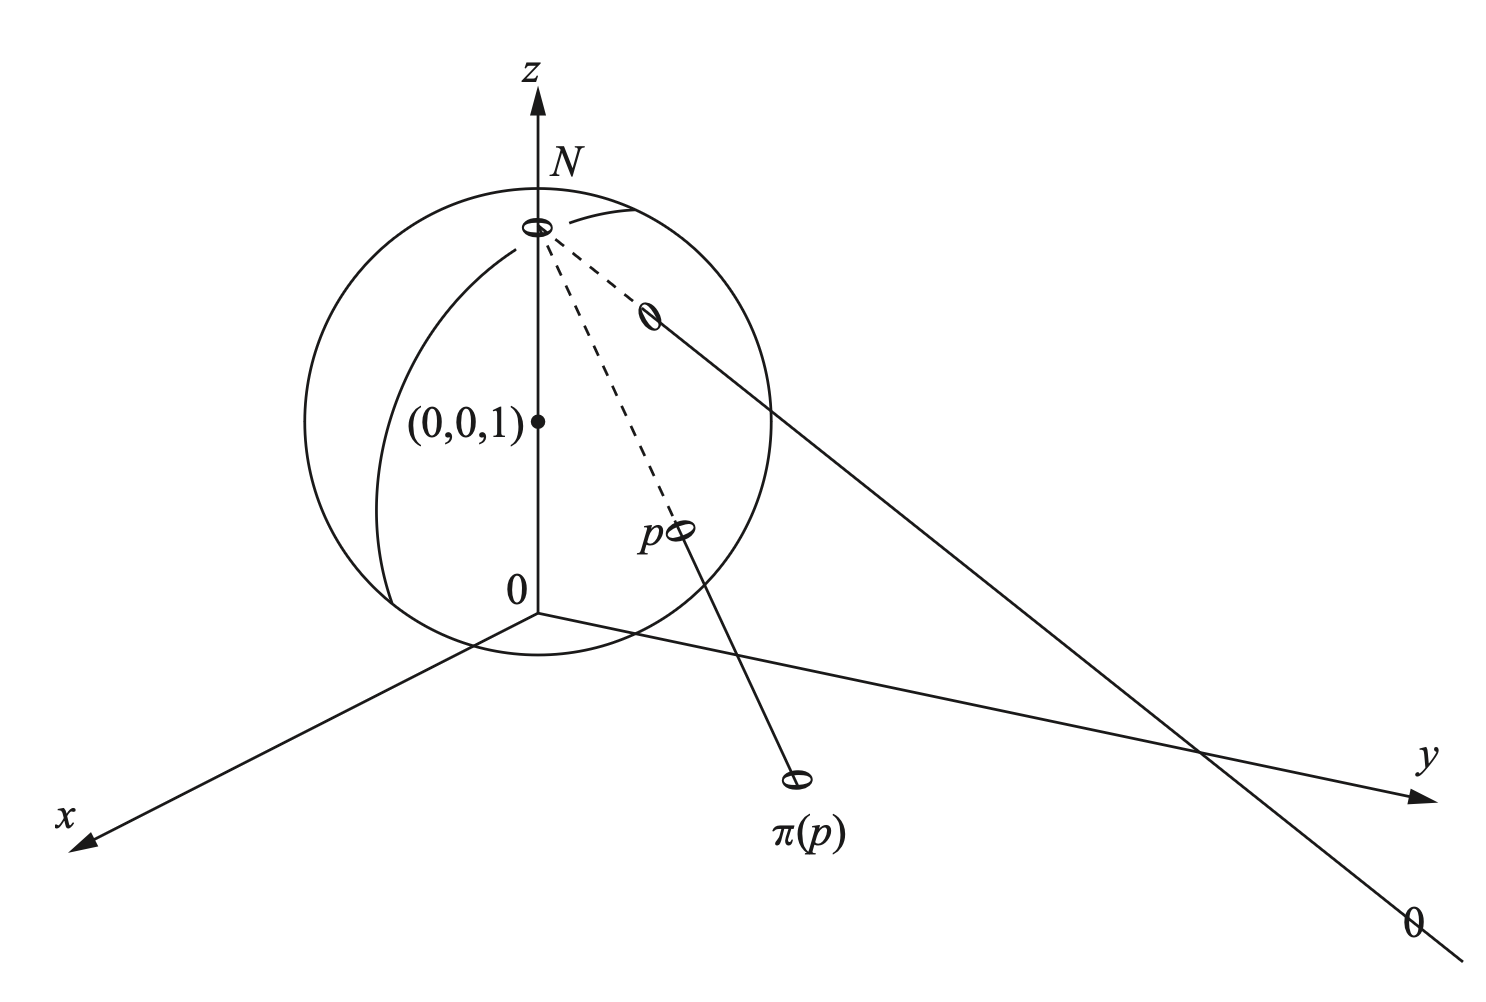
\includegraphics[scale=0.5]{imagenes/4.png}
    \end{figure}

    \begin{enumerate}
        \item Pruebe que $\pi^{-1}: \mathbb{R}^2 \rightarrow S^2$ está dada por
        $$
x=\frac{4 u}{u^2+v^2+4}, \quad y=\frac{4 v}{u^2+v^2+4}, \quad z=\frac{2\left(u^2+v^2\right)}{u^2+v^2+4} .
$$
\begin{sol} Comenzamos parametrizando los puntos $N = (0, 0, 2)$ y $p = (x, y, z)$, con la expresión: $$ \left\{\begin{array}{l} x(t) = x_0 + t(x - x_0) \\ y(t) = y_0 + t(y - y_0) \\ z(t) = z_0 + t(z - z_0) \end{array}\right. \implies \left\{\begin{array}{l} x(t) = t(x) \\ y(t) = t(y ) \\ z(t) = 2 + t(z - 2) \end{array}\right. $$ Ahora bien, buscamos encontrar el valor $t$ en donde la parametrización instersecta el plano $xy$. Es decir $z=0$, entonces con la tercera ecuación tenemos $$t = \frac{2}{2-z}.$$ De esto, obtenemos: 
    $$ x(t)=\frac{2x}{2-z} $$ y $$ y(t)=\frac{2y}{2-z} $$

    Si $(u,v)$ es el punto de intersección con el plano, tenemos: 
    $$ u=\frac{2x}{2-z} \implies x=\frac{u(2-z)}{2}$$ y $$ v=\frac{2y}{2-z}\implies y=\frac{v(2-z)}{2} $$

    Entonces, ya tenemos: 
    \begin{align*}
        x^2+y^2+(z-1)^2&=1\\
        \left(\frac{u(2-z)}{2}\right)^2+\left(\frac{v(2-z)}{2}\right)^2+(z-1)^2 &= 1\\
        \frac{u^2(2-z)^2}{4}+\frac{v^2(2-z)^2}{4}+(z-1)^2 &= 1\\
        u^2(2-z)^2+v^2(2-z)^2+4(z-1)^2 &= 4\\
        (4-4z+z^2)(u^2+v^2)+4(z^2-2z+1) &= 4\\
        (4u^2-4zu^2+z^2u^2)+(4v^2-4zv^2+z^2v^2) + 4z^2-8z+4 &= 4 \\
        (u^2+v^2+4)z^2+(-4u^2-4v^2-8)z+(4u^2+4v^2+4) &= 4\\
        (u^2+v^2+4)z^2-4(u^2+v^2+2)z+4(u^2+v^2) &= 0\\
    \end{align*}
    Despejamos para $z$, usando \textit{Mathematica}:
    \begin{figure}[H]
        \centering 
        
\includegraphics[scale=0.4]{imagenes/5.png}
    \end{figure}
        Entonces, en $x$ tenemos: 
        \begin{figure}[H]
            \centering 
            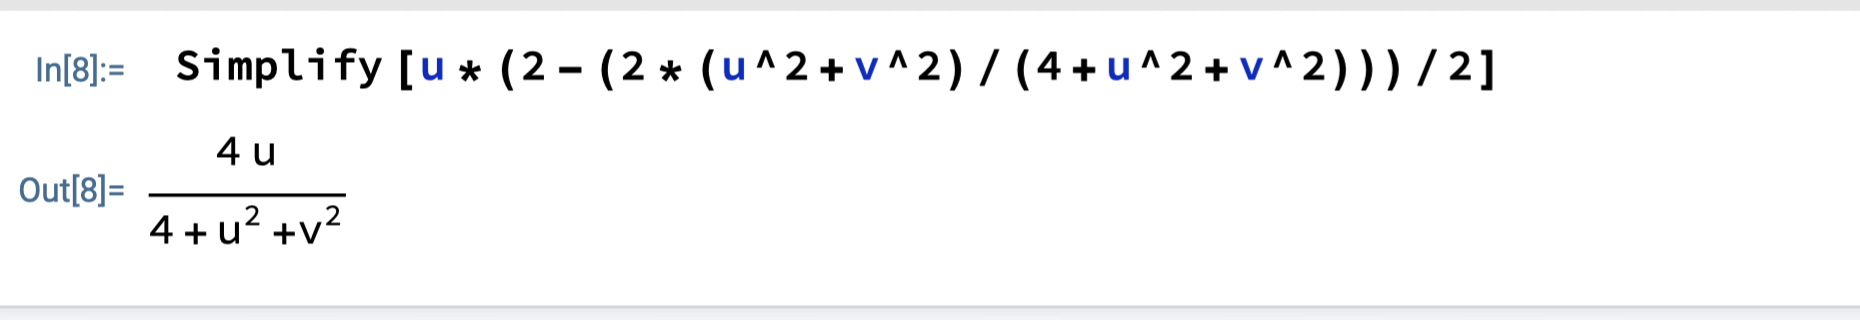
\includegraphics[scale=0.4]{imagenes/6.png}
        \end{figure}
        En $y$: 
        \begin{figure}[H]
            \centering 
            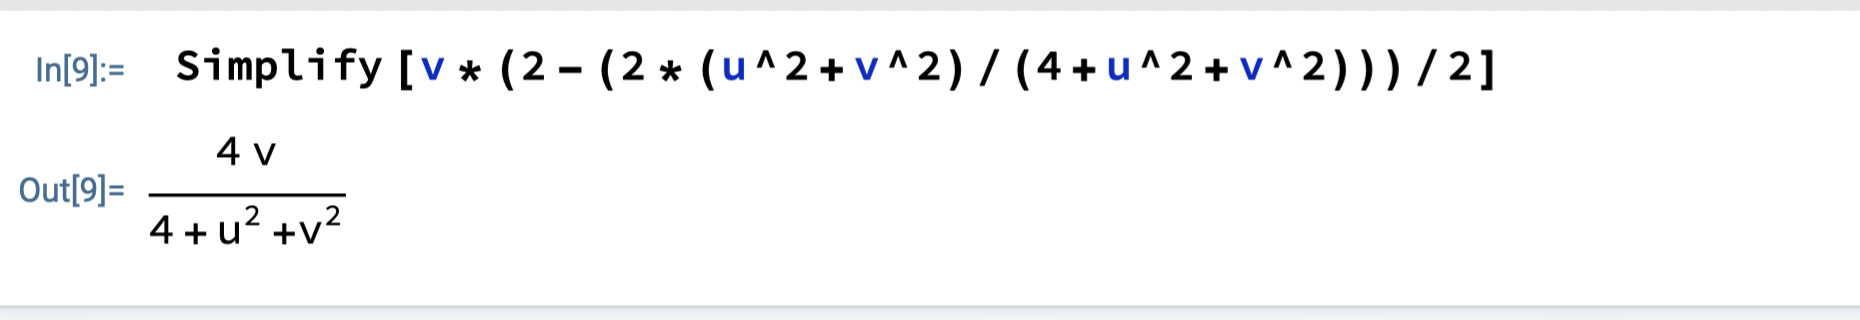
\includegraphics[scale=0.4]{imagenes/7.png}
        \end{figure}
        Y por lo tanto, 
        $$
x=\frac{4 u}{u^2+v^2+4}, \quad y=\frac{4 v}{u^2+v^2+4}, \quad z=\frac{2\left(u^2+v^2\right)}{u^2+v^2+4} .
$$

\end{sol}

        \item Muestre que es posible, usando la proyección estereográfica, cubrir la esfera con dos cartas locales.
        \begin{sol}
            Analizamos la parametrización anterior para que sea una carta.
            $$\pi^{-1}(u,v)=\left(\frac{4u}{u^2+v^2+4}, \frac{4v}{u^2+v^2+4}, \frac{2(u^2+v^2)}{u^2+v^2+4}\right)$$
            \begin{itemize}
                \item $\pi^{-1}$ es diferenciable. Analizamos la existencia de las derivadas parciales y también verificamos que son continuas. 
                \begin{figure}[H]
                    \centering 
                    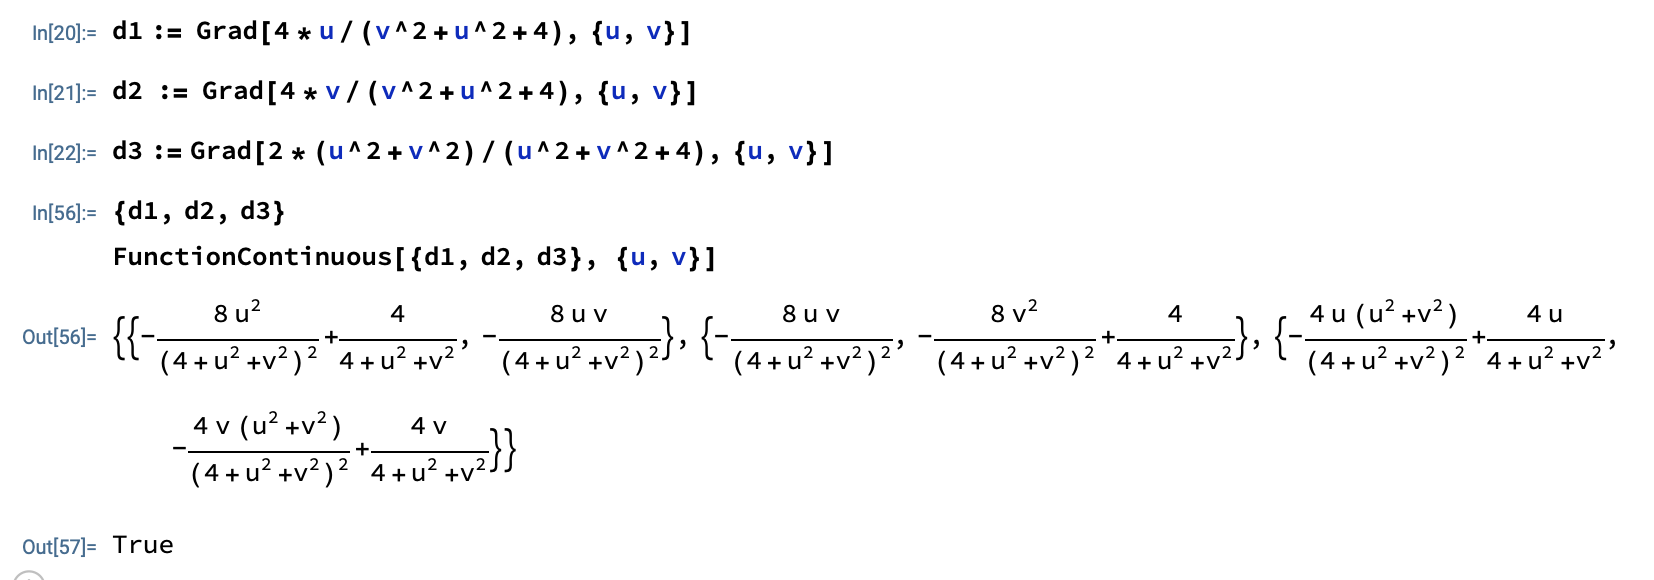
\includegraphics[scale=0.5]{imagenes/8.png}
                \end{figure}

                \item $\pi^{-1}$ es un homomorfismo. Nótese que $f$ es continua, porque sus componentes lo son. La propiedad de ser biyectiva (inyectividad y sobreyectivad) es directa por la forma en que definimos $\pi^{-1}$. 
                \item La derivada $dx_1:\mathbb{R}^2\to T_p(\mathbb{R}^3)$ es inyectiva para cada $q\in U$. Verificamos que los vectores los vectores de derivadas parciales $x_u,v_v$ son linealmente independientes, es decir el producto cruz no es igual a cero. Lo cual verificamos a continuación: 
                \begin{figure}[H]
                    \centering 
                    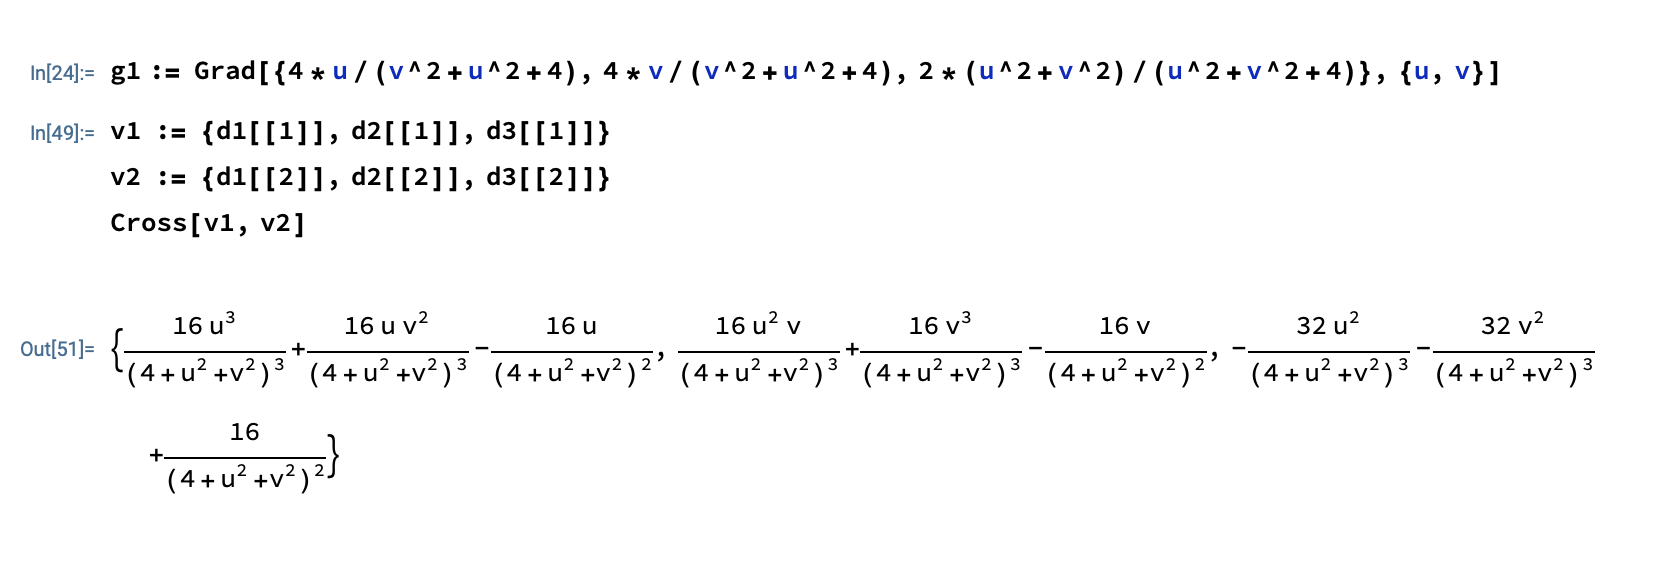
\includegraphics[scale=0.5]{imagenes/9.png}
                \end{figure}
            \end{itemize}
            
            Ahora, la otra carta la podemos generar con el polo sur $S=(0,0,-2)$ y el procedimiento es análogo. 
        \end{sol}
    \end{enumerate}

\end{problema}

\begin{problema}
    Sea $S^2=\left\{(x, y, z) \in \mathbb{R}^3 ; x^2+y^2+z^2=1\right\}$ la esfera unitaria y sea $A: S^2 \rightarrow S^2$ el mapa antipodal $A(x, y, z)=(-x,-y,-z)$. Pruebe que $A$ es un difeomorfismo.
    \begin{dem}
        Para demostrar este enunciado, nos apoyamos en la siguiente definición vista en clase:
        \begin{cajita}
Dos superficies regulares $\mathrm{S}_1$ y $\mathrm{S}_2$ en $\mathbb{R}^3$ son difeomorfas si existe una aplicación biyectiva diferenciable $\varphi: S_1 \rightarrow S_2$, con inversa $\varphi^{-1}: S_2 \rightarrow S_1$ también diferenciable.
        \end{cajita}
        $S^2$ ya se había demostrado en clase que es una superficiente regular. A probar: (1) Biyectividad (2) $A$ es diferenciable (3) Inversa de $A$ es diferenciable. 
        Sea entonces, 
        \begin{itemize}
            \item Biyectividad. Hay que probar que $A$ es inyectivo y sobreyectivo. \begin{itemize}
                \item Inyectividad. Sea
                \begin{align*}
                    A(x,y,z) &= A(x',y',z')\\
                    (-x, -y, -z) &= (-x', -y', -z')\\
                    (x, y, z) &= (x', y', z')\\
                \end{align*}
                \item Sobreyectividad. Cada $(x,y,z)\in S^2$, tenemos que $A(-x,-y,-z)= (x,y,z)$ entonces cada punto en $S^2$ tiene una preimagen bajo $A$. 
            \end{itemize}
            \item $A$ es diferenciable. Para esto, nos apoyamos en la siguiente definición vista en clase: 
            \begin{cajita}
                Sea $f: S_1 \rightarrow S_2$ una aplicación entre superficies regulares $S_1$ y $S_2$. Diremos que $f$ es diferenciable si para cualesquiera parametrizaciones $\mathbf{x}: U \subseteq \mathbb{R}^2 \rightarrow S_1$ y $\mathbf{y}: V \subseteq \mathbb{R}^2 \rightarrow S_2$, con $f \circ \mathbf{x}(U) \subseteq \mathbf{y}(V)$, se tiene que la aplicación $\mathbf{y}^{-1} \circ f \circ \mathbf{x}: U \rightarrow V$ es diferenciable.
            \end{cajita}
            Sean $\mathbf{x}_1:U_1\to S^2$ y $\mathbf{x}_2:U_2\to S^2$ parametrizaciones tales que $A(\mathbf{x}_1(U_1))\subset \mathbf{x}_2(U_2)$. Entonces debemos probar que $$ \mathbf{x}_2^{-1}\circ A\circ \mathbf{x}_1:U_1\to U_2 $$ es diferenciable.

            Para esto, 
            \item Inversa diferenciable. Sea $A(A(x,y,z))=A(-x,-y,-z)=(x,y,z)$, lo que implica que $A^{-1}=A$ y por lo tanto, el inciso anterior aplica aqui también, mismo argumento. Inversa diferenciable. 

            
        \end{itemize}
    \end{dem}
    
\end{problema}

\begin{problema}
    Sea $S \subseteq \mathbb{R}^3$ una superficie regular y sea $\pi: S \rightarrow \mathbb{R}^2$ el mapa que toma cada punto $p \in S$ y lo lleva a su proyección ortogonal sobre $\mathbb{R}^2$. ¿Es $\pi$ diferenciable?
    \begin{sol}
        Primero, definimos a la proyección ortogonal como $\pi:S\subseteq\mathbb{R}^3\to \mathbb{R}^2$ y $p=(x,y,z)\in S$ tal que: 
        $$\pi(p)=\pi(x,y,z)=(x,y)$$

        Usando la definición vista en el problema anterior, sean $\mathbf{x}_1:U_1\subseteq \mathbb{R}^2\to S$ y $\mathbf{x}_2:U_2\subseteq\mathbb{R}^2\to \mathbb{R}^2$ parametrizaciones tales que $\pi(\mathbf{x}_1(U_1))\subset \mathbf{x}_2(U_2)$. Entonces debemos probar que $$ \mathbf{x}_2^{-1}\circ \pi \circ \mathbf{x}_1:U_1\to U_2 $$ es diferenciable. Sea cualesquiera parametrizaciones de la forma
        \begin{align*}
            x_1(u,v) &= (x(u,v),y(u,v),z(u,v))\\
            x_2(u,v) &= (u,v) \implies x_2^{-1}(u,v) = (u,v)
        \end{align*}
        Entonces, 
        \begin{align*}
            \mathbf{x}_2^{-1}\circ \pi \circ \mathbf{x}_1(u,v) &=  \mathbf{x}_2^{-1}(\pi (\mathbf{x}_1(u,v)))\\
            &= \mathbf{x}_2^{-1}(\pi (x(u,v),y(u,v),z(u,v)))\\
            &= \mathbf{x}_2^{-1}(x(u,v),y(u,v))\\
            &=(x(u,v),y(u,v))\\
        \end{align*}
        Es decir que cualquier parametrización $x_1$ y $x_2$ funciona de la forma propuesta, solo basta asegurar que sus componentes sean diferenciables. Por lo tanto, $\pi$ es diferenciable. 
    \end{sol}
\end{problema}

\begin{problema}
    Sea 
    \begin{enumerate}
        \item Mostrar que el paraboloide $z=x^2+y^2$ es difeomorfo al plano.
        \begin{sol}
            Sea $S=\{(x,y,z)\in \mathbb{R}^3| z=x^2+y^2\}$ una superficie regular, 
            \begin{figure}[H]
                \centering 
                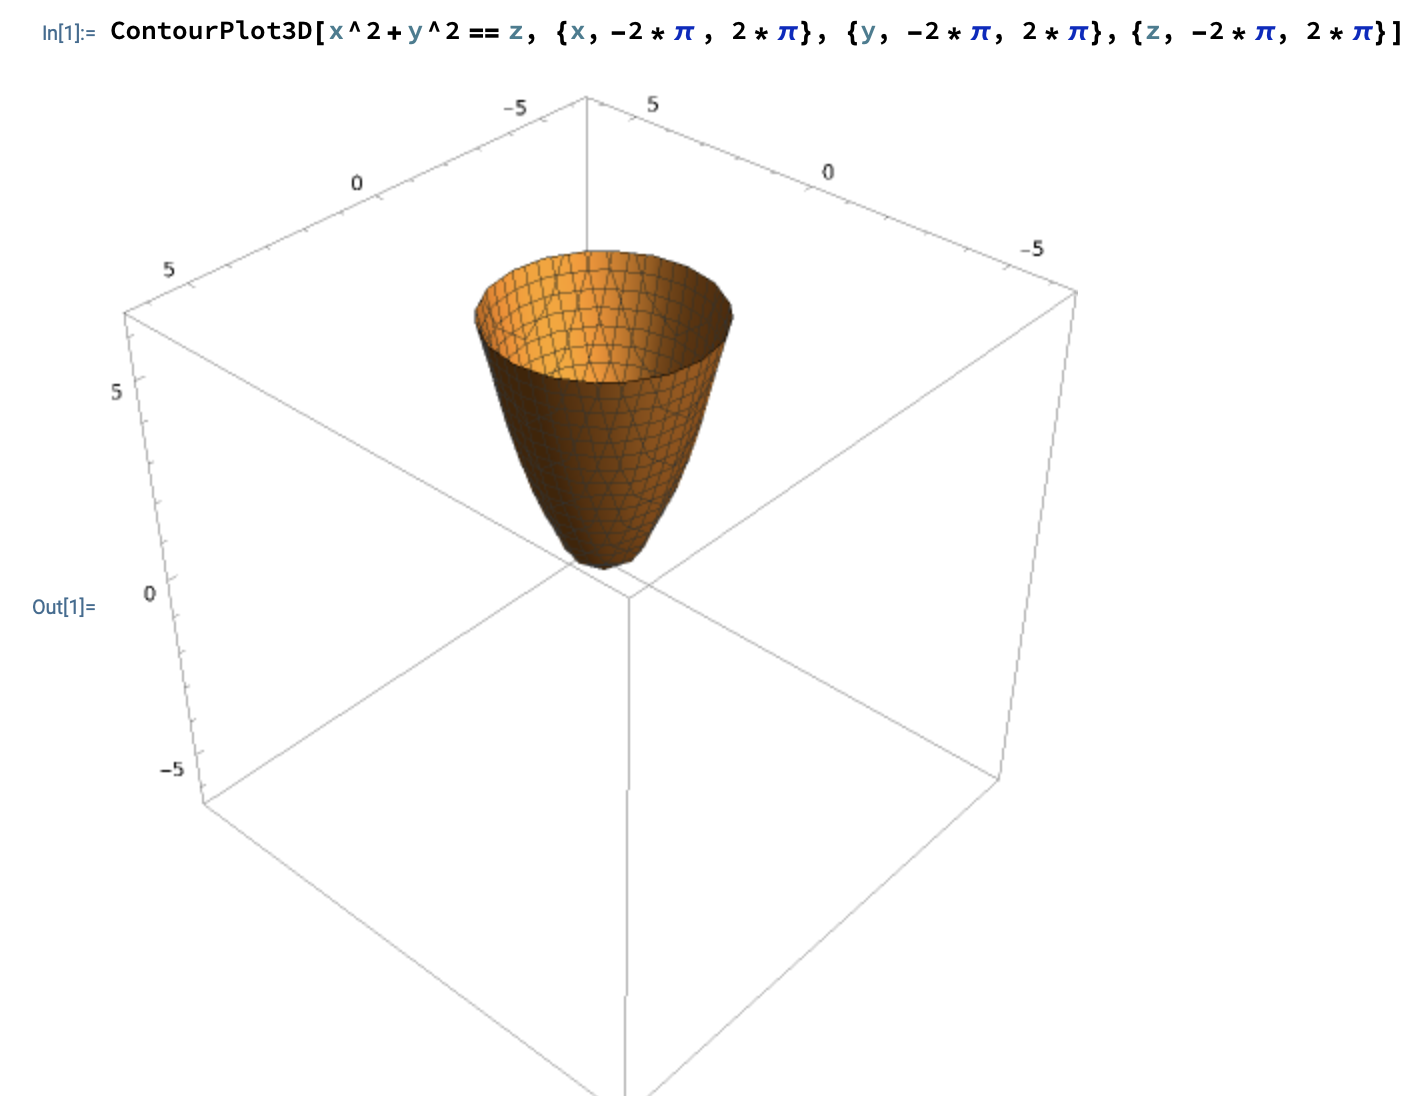
\includegraphics[scale=0.5]{imagenes/2.png}
            \end{figure}
            Sea $f:\mathbb{R}^2\to S, f(u,v)=(u,v,u^2+v^2)$. A probar: $f$ es un difeomorfismo $\iff$ es diferenciable, biyectivo e inversa diferenciable.
            \begin{figure}[H]
                \centering 
                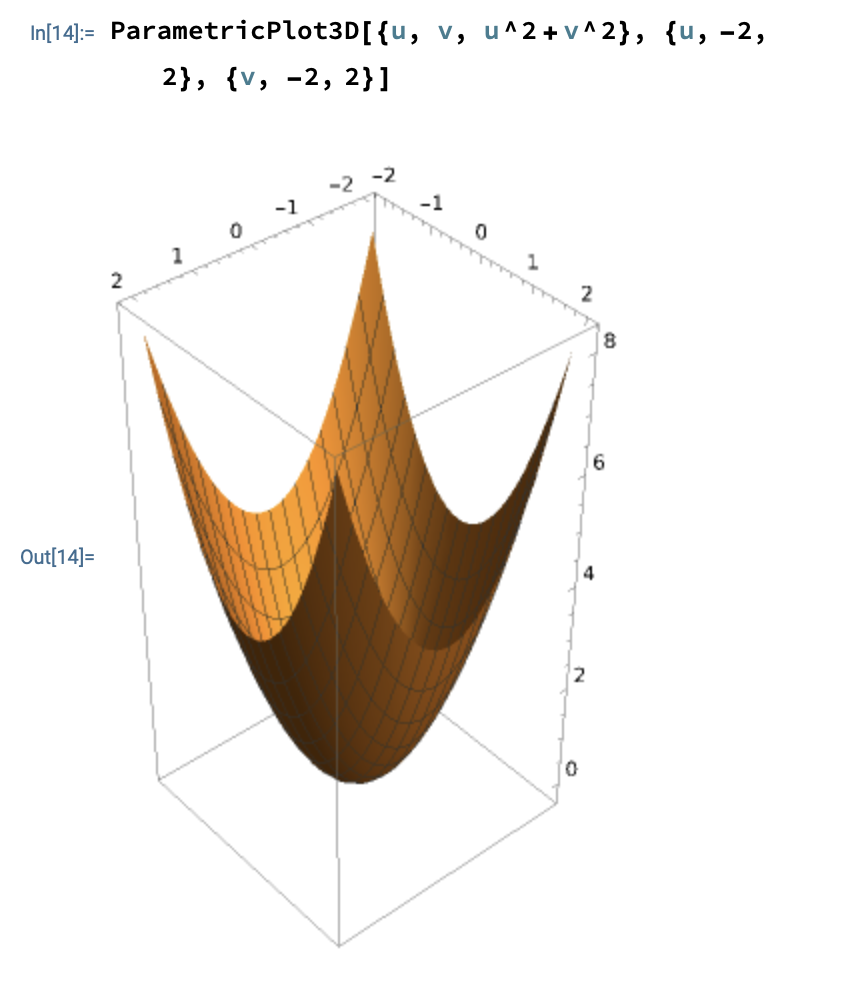
\includegraphics[scale=0.5]{imagenes/3.png}
            \end{figure}
            Dicha parametrización es diferenciable por la definición (mismo argumento del Problema 7, sus componentes son diferenciables) y es biyectiva por: 
            \begin{enumerate}
                \item Inyectiva. 
                \begin{align*}
                    f(x,y)&= f(x',y')\\
                    (x,y,x^2+y^2) &= (x',y',x'^2+y'^2)
                \end{align*} 
                y de esto, concluimos 
                $$x=x',y=y'\implies (x,y)=(x',y')$$
                \item Sobreyectiva. Sea $(z,y,z)\in S,\exists (x,y)\in \mathbb{R}^2$ tal que se cumple la regla de asignación. 
            \end{enumerate}
            Entonces tenemos que $f$ es un mapa inyectivo diferenciable. Solo falta encontrar la inversa, la cual es la misma del problema 7, $$\pi(x,y,z)=(x,y)$$
            la cual es diferenciable. Por lo tanto el paraboloide $z=x^2+y^2$ es difeomorfo al plano.
        \end{sol}
        \item Construir un difeomorfismo entre el elipsoide $\frac{x^2}{a^2}+\frac{y^2}{b^2}+\frac{z^2}{c^2}=1$ y la esfera unitaria $S^2: x^2+y^2+z^2=1$.
        \begin{sol}

            Sea $E$ el elipsoide y $S^2$ la esfera.Definimos un mapa $f: E \rightarrow S$:  $$ f(x,y,z) = \left(\frac{x}{a},\frac{y}{b},\frac{z}{c}\right). $$ A probar: $f$ es un difeomorfismo $\iff$ es diferenciable, biyectivo e inversa diferenciable. Nótese que la parametrización es diferenciable por la definición (mismo argumento del Problema 7, sus componentes son diferenciables), ya que sus componentes son diferenciables. Entonces verificamos que es biyectiva: 
            \begin{enumerate}
                \item Inyectiva. 
                \begin{align*}
                    f(x_1,y_1,z_1) &= f(x_2,y_2,z_2)\\
                    \left(\frac{x_1}{a},\frac{y_1}{b},\frac{z_1}{c}\right) &= \left(\frac{x_2}{a},\frac{y_2}{b},\frac{z_2}{c}\right)\\
                    \left(\frac{x_1}{a},\frac{y_1}{b},\frac{z_1}{c}\right) &= \left(\frac{x_2}{a},\frac{y_2}{b},\frac{z_2}{c}\right)
                \end{align*}
                \item Sobreyectiva. Sea $(x’,y’,z’) \in S$. Entonces, $$ (x’)^2 + (y’)^2 + (z’)^2 = 1. $$ Let $(x,y,z) = (ax’,by’,cz’)$. De mesto, $$ \left(\frac{x^2}{a^2}+\frac{y^2}{b^2}+\frac{z^2}{c^2}\right) = 1, $$ so $(x,y,z) \in E$. Además, $$ f(x,y,z) = f(ax’,by’,cz’) = \left(\frac{ax’}{a},\frac{by’}{b},\frac{cz’}{c}\right) = (x’,y’,z’). $$ Entonces para cada punto en $S$, existe un punto en  $E$ tal que se cumple la regla de asignación. 
            \end{enumerate}

Por otra parte, su inversa es $$ f^{-1}(x,y,z)=(ax,by,cz), $$
la cual es diferenciable, también. 

        \end{sol}
        
    \end{enumerate}
\end{problema}
%---------------------------
%\bibliographystyle{apa}
%\bibliography{referencias.bib}

\end{document}